\chapter[\'Etude en clinique]{\'Etude avec utilisation du test
  d'écoute en clinique psychiatrique}

Nous savons que la musicothérapie est de plus en plus intégrée dans
les milieux psychiatriques.
L'objectif ici est de vérifier l'hypothèse évoquée et qui est celle de savoir s'il est possible d'estimer, après un travail 
musicothérapeutique, la transformation de l'écoute mesurée chez le
patient.
Les tests ont été faits en avril, mai, juin, juillet, septembre et octobre 2017.

\section{Cadre de travail}

 La Privatklinik
de Meiringen est  spécialisée en
addictologie dans le canton de Berne. Elle dispose d'une capacité de 195 lits, 33 médecins et
psychologues, secondés par 177 soignants qui assurent les soins du
patient.




\subsection{Les patients: description}


-Moyenne d'âge:  entre 20 à 60 ans, masculin et féminin quasi égale.


-Pathologies:  burnout, dépendances, dépression.

-Temps de séjour: 3 à 6 semaines, voire plusieurs mois.
-Fréquence du traitement en musicothérapie: 1x par semaine pendant
50mn à 60mn.
-Le type de musicothérapie: habituelle dans ce contexte.
Ont été  exclu l'écoute avec casques et  musiques traitées chez Tomatis.
-Contexte de la clinique: contexte habituel d'une prise en
charge en clinique psychiatrique 
par les médecins et  les psychologues.
En plus, diverses thérapies sont proposées: physio--,ergo--,
art--,musico--,corporel--, zoo--  (chien/ cheval)  ainsi
que par les  ateliers de créativité sur le bois, la terre, la laine.  


\section{Design d'étude}

Mise en place:

Un groupe d'intervention et un groupe de contrôle ont été constitués.
La direction de la clinique ayant accepté l'étude, le personnel soignant et tout le
corpus des thérapies créatives ont  été
informés au préalable.

Les patients ont été avertis par un
court entretien individuel réalisé généralement par la musicothérapeute Regula Lehman  \footnote{Regula
  Lehmann, musicothérapeute  à 90\%  à la clinique de Meiringen.} et par  une
feuille explicative de notre démarche sur  l'évaluation de l'écoute et
sur
l'hypothèse de la transformation de cette écoute lors de leur 
séjour en thérapie. \emph{Information für Mitwirkende an der klinischen
  Studie\  ``Evaluierung des aktiven Hörvermögens" }.
Les patients étaient libres de participation. Ceux qui
l'ont fait, ont signé leur accord  officiellement à chaque fois  \emph{``Eine schriftliche Einbewilligung zum
Test"} avant de passer les deux types de tests dont nous nous sommes
occupés: Le questionnaire/test WHO QOL-Bref et le test d'écoute.

 
 
 

\section{Instruments de mesure: le WHO QOL - Bref et le test d'écoute}
 Nous redonnons quelques précisions sur le WHO QOL-Bref mais ne
 reviendrons pas sur le test d'écoute, suffisamment décrit au chapitre 8.

\subsection{Le WHO QOL - Bref}

Nous avons utilisé et fait en parallèle le test WHOQO-Bref avant et
après pour avoir une variable supplémentaire pour confirmer en
parallèle supposée de l'action de la musicothérapie sur une éventuelle modification de l'écoute.  C'est une
version test de 1997 issue du Programme sur la santé mentale,
Organisation mondiale de la santé, Genève. Il y a 26 questions, que le
patient a rempli lui-même en présence du thérapeute, avant ou après le test
d'écoute. La durée pour les remplir a varié de 8 à 10 minutes en
moyenne. 

Il y a quatre domaines testés : physique, psychologique, relations sociales et environnement.
\begin{enumerate}
	\item  Le domaine de la perception physique comprend l' activité quotidienne// la dépendance et/ou l'assistance médicale// la fatigabilité, l'énergie//la mobilité// la douleur// le sommeil// la capacité de travail//
	
		 \item Le domaine psychologique :  image de soi, apparence// ressentis positifs et négatifs// estime de soi// spiritualité, croyances personnelles, religion// mémoire et concentration, apprentissage, pensée.
		
			\item Le domaine des relations sociales : relations personnelles// soutien social// vie sexuelle.
			
			\item Le domaine de l'environnement : l'environnement domestique et  physique (pollution, bruit, trafic, climat)// la situation financière//  la liberté, la sécurité physique et morale// l'accessibilité et qualité de la santé// les opportunités de détente, loisirs et d'acquisition d'informations// le transport// 
		\end{enumerate}
		
	




        	
        \subsection{Technique d'intervention:}


       
\begin{itemize}
	\item Un groupe A de patients en musicothérapie : un
          test avant leur prise en charge en musicothérapie; avec un questionnaire
          WHOQOL.
          
          .un 2\ieme\ test et un questionnaire WHOQOL : après 4 semaines de
          clinique.
          
	\item Un groupe B de contrôle sans musicothérapie,
	toujours dans le même contexte, c.à.dire en clinique, avec le suivi et les mêmes protocoles que l'autre groupe. Un premier test avant
 puis un deuxième test, avec les questionnaires WHOQOL, après 4 semaines. 
\end{itemize}

 Par ordre chronologique:
 
\begin{enumerate} 
        \item Un test d'écoute, un entretien et un questionnaire
          WHOQOL pour les groupes A et B.
        \item Séances de musicothérapie, actives ou réceptives (1x par
          semaine) pour le groupe A.
        \item Deuxième test d'écoute, entretien et questionnaire
          WHOQOL pour les groupes A et B.
\end{enumerate}

	
	
	Durée des tests : Chaque test d'écoute a une durée  moyenne de
        60 minutes par patient. Pour chacun, nous avons donc réalisé
        en tout au minimum deux heures de tests d'écoute avec un
        entretien (2x15') à chaque fois.
        Le questionnaire WHOQOL (2x10')  a été remplis par les
        patients avant le début du séjour en clinique et après, lors
        de leur sortie.
        
       
      
        Nombre de tests réalisés:
        
     Nous avons réalisé en tout 44 tests d'écoute et 25 questionnaires 
     WHOQOL-Bref.
     
     Sur les tests d'écoute:
     -16 tests d'écoute non-valides car 
     incomplets
     -18 tests d'écoute valides de patients pour le groupe B, sans le suivi en 
     musicothérapie
     -10 tests d'écoute valides de patients pour le groupe A, avec le
     suivi en musicothérapie.

     
     Sur les questionnaires à remplir: 
     -18 questionnaires WHOQOL valides
     -  7 questionnaires non valides, car non complets ou vides.
     
     
          
 
 
 	
 	
       

 	
 	\section{Un graphique: déroulement de l'étude avec un groupe
          de contrôle et un groupe d'intervention}





                                      Patients souffrant de dépression, burnout
                                               en séjour dans la
                                               clinique, répartis en
                                               deux groupes.
                                             

\begin{figure}
\centering
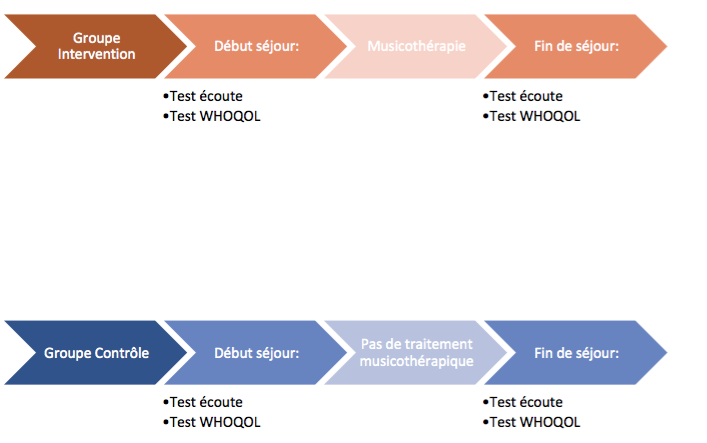
\includegraphics[width=0.7\linewidth]{images/Groupecontrole.png}
\caption[Schéma du déroulement]{Déroulementde l'étude avec les
         deux groupes}
       
\label{groupecontroleimage1}
\end{figure}

\begin{figure}
\centering
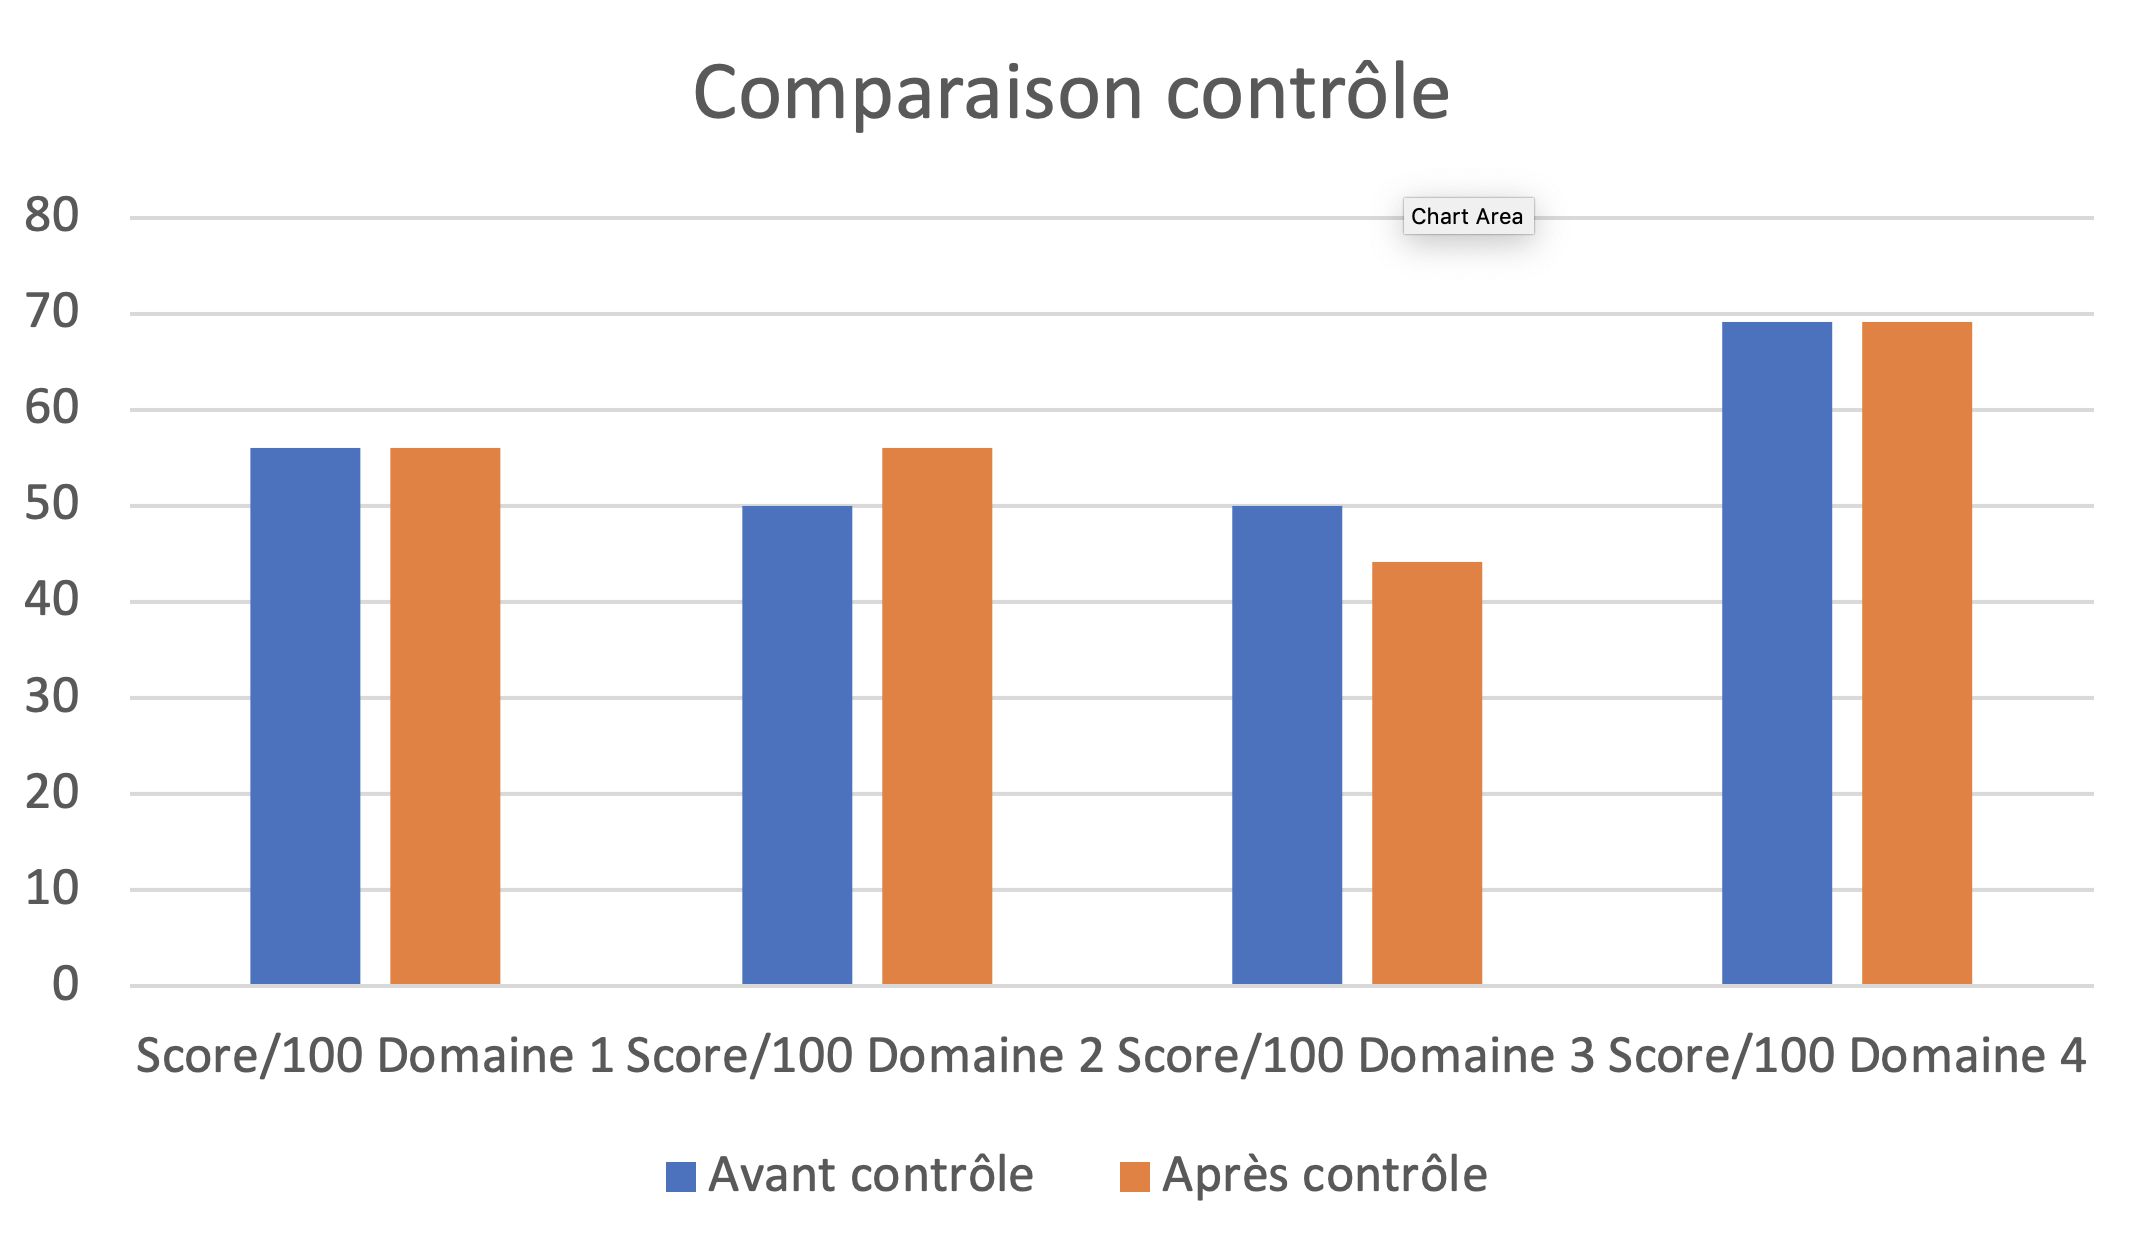
\includegraphics[width=0.7\linewidth]{images/Compcontrole.png}
\caption[Schéma du déroulement]{Déroulementde l'étude avec les
         deux groupes}
       
\label{groupecontroleimage1}
\end{figure}

\begin{figure}
\centering
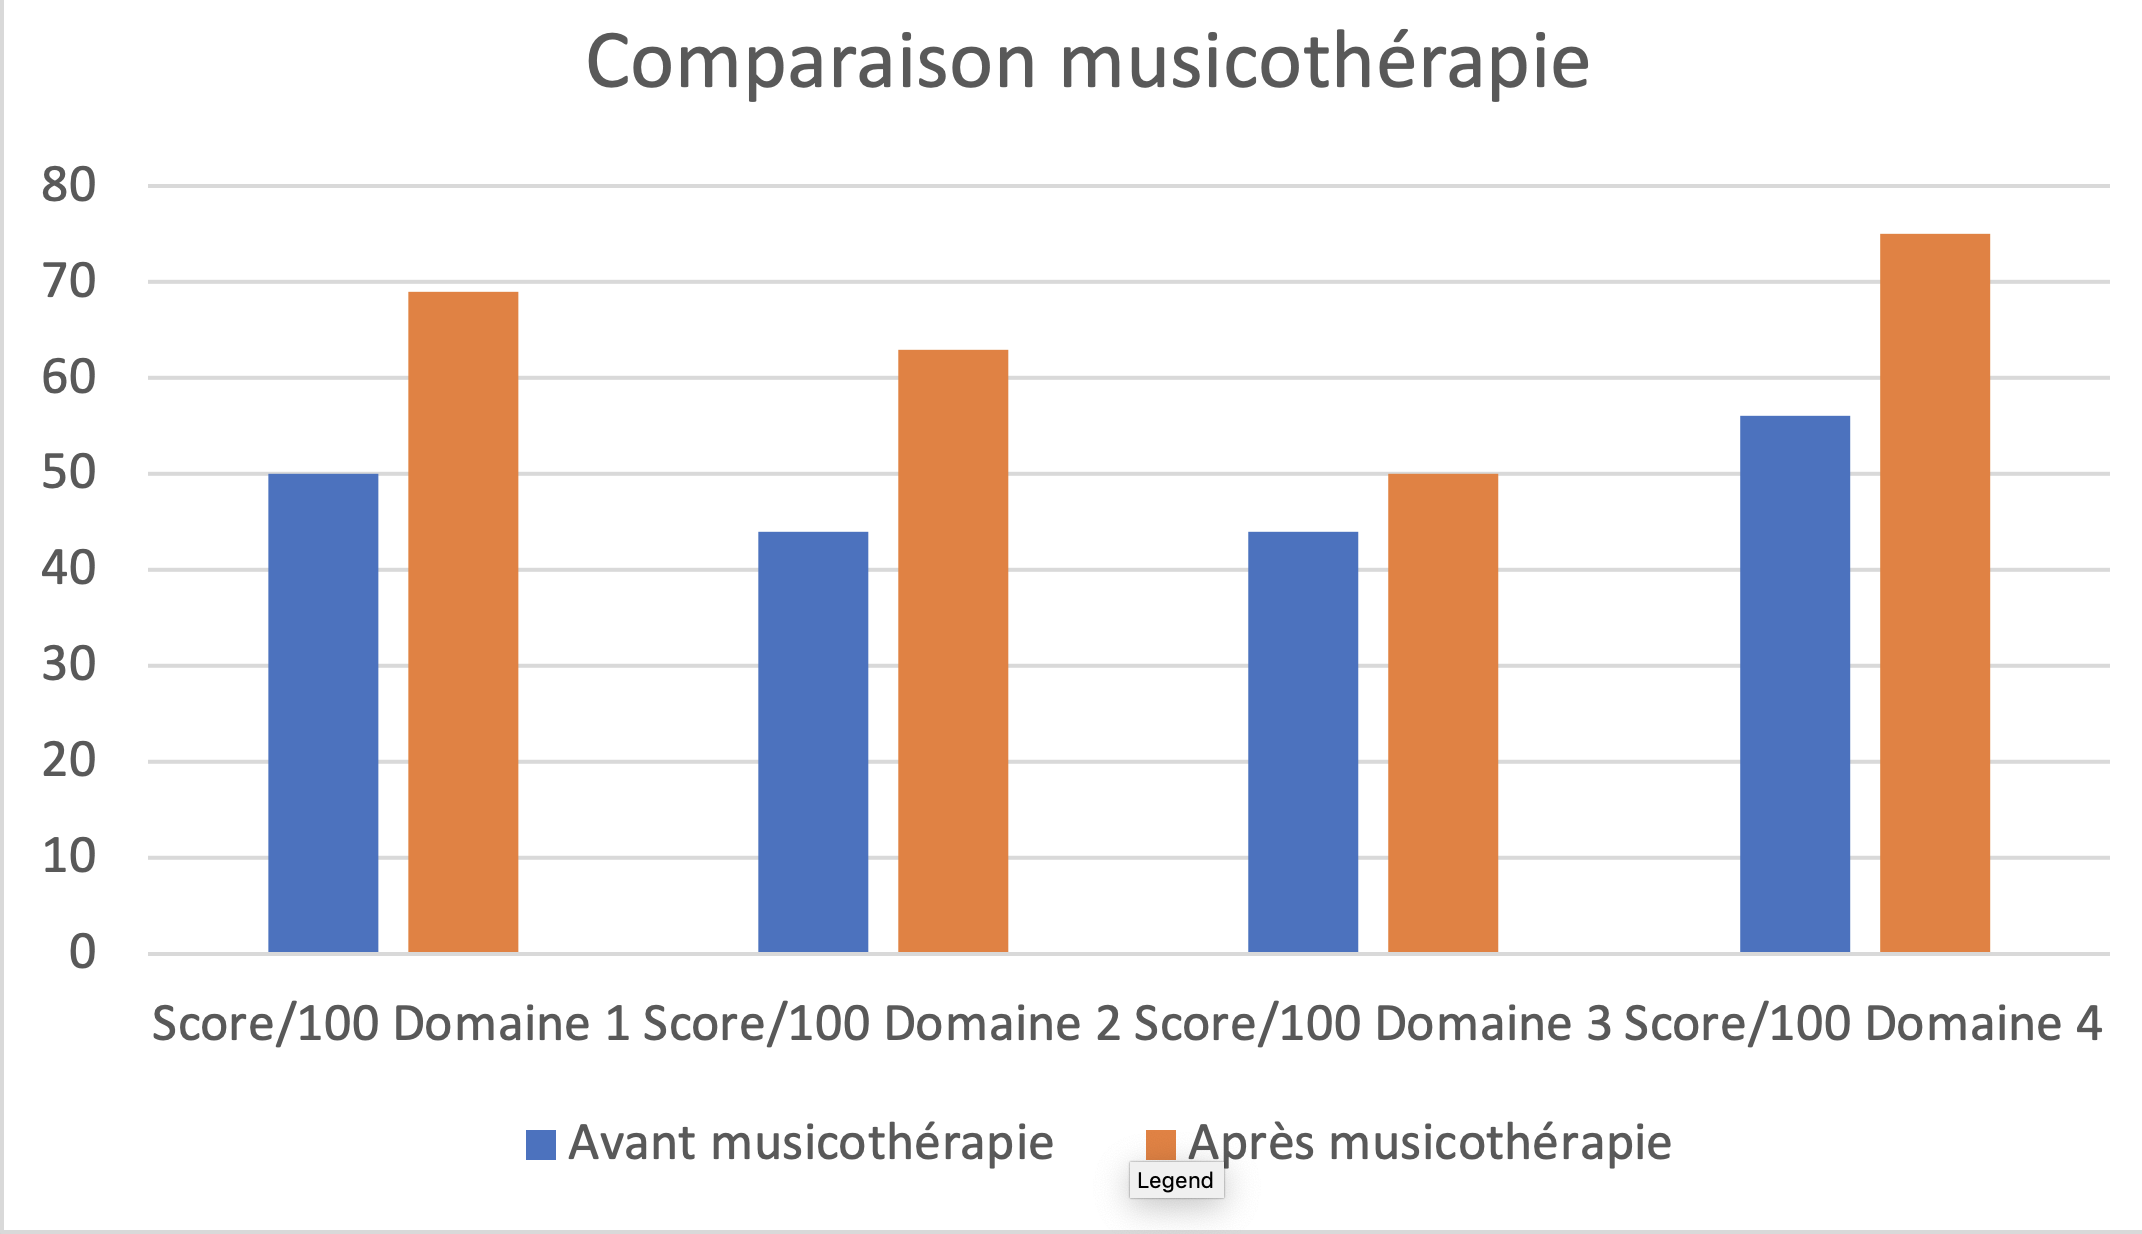
\includegraphics[width=0.7\linewidth]{images/Compmusico.png}
\caption[Schéma du déroulement]{Déroulementde l'étude avec les
         deux groupes}
       
\label{groupecontroleimage1}
\end{figure}



        
        Groupe de contrôle                                                    Groupe
                                                                                     d'intervention

1°test d'écoute avant thérapie, début de séjour           Idem+musicoth.

1°test WHO QOL-Bref

                                                                                     Idem+musicoth.
2°Test en fin de thérapie, fin de séjour
2°Test WHO QOL-Bref
 



\section{Les 3 zones avec leur résonance en musicothérapie et en
  psychologie}


	Informations croisées avec les informations récoltées par les 3 
          zones du test d'écoute:
          
Les paramètres utilisés en musicothérapie trouvent leur lien avec les
3 zones d'interprétation psychologique du test d'écoute.
\begin{itemize}
 \item Le rythme, tempo, puls  =  Z.1: le physique, le corps, l'incorporéisation et
l'intégration du rythme,
la posture d'écoute.

\item La voix, le timbre, la mélodie =  Z.2:  l'expression vocale, la communication,
l'émotionnel, la sensibilité, l'affect.

\item La justesse= l'harmonie (consonance, dissonance) et l'improvisation = Z.3:  la créativité, l'interprétation, la
résonance, la musicalité, la motivation, le non-verbal (
l'intraduisible en mot), l'espace.
\end{itemize}

Si nous référons à la conception antique des chakras ainsi qu'au sens de la
topique de Freud (ça, moi et surmoi), nous trouvons des correspondances
avec les trois zones entre les
fréquences et ``la distribution de l'énergie pulsionnelle'' ou entre
les 
``caractéristiques du son et l'énergie instinctuelles''. (B.Auriol, La
clef des sons).
``La mélodie est la seule forme musicale de la décharge individuelle, car le rythme est le moteur, pré-musical, et l'harmonie, supra-individuelle `` (Mosonyi, 1935, cité par Michel, 1965).

 

\begin{figure}
	\centering
	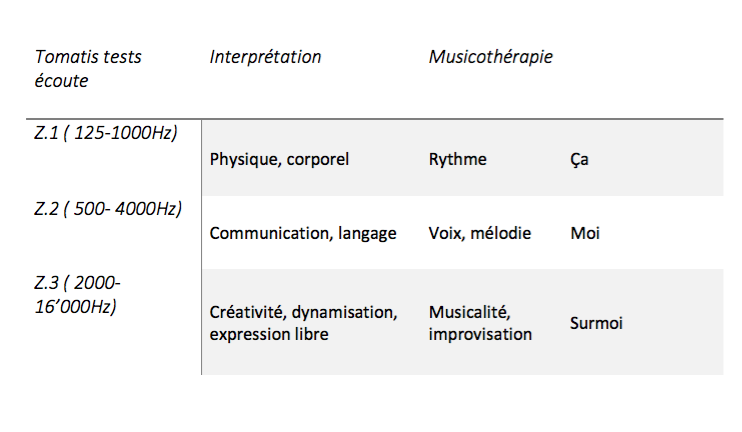
\includegraphics[width=0.7\linewidth]{images/testinterpmusico}
	\caption[ L'interprétation des 3 zones et leur correspondance
        en musicothérapie]{Graphique. interprétation des 3 zones du
          test et leur correspondance en musicothérapie}
       
	\label{graphiquecolonnetestmusico}
      \end{figure}











      


  

\section{Comparaison de deux tests d'écoute, avant et après la musicothérapie: 1°Test--2°test, considérations générales}
	
 	
\subsection{Le patient M avant musicoth.}

 	Le patient M souffre de Burnout. Vif, il se montre très
        intéressé pour participer à l'étude.
 
 	
 	\begin{figure}[tbh]
 		\centering
 		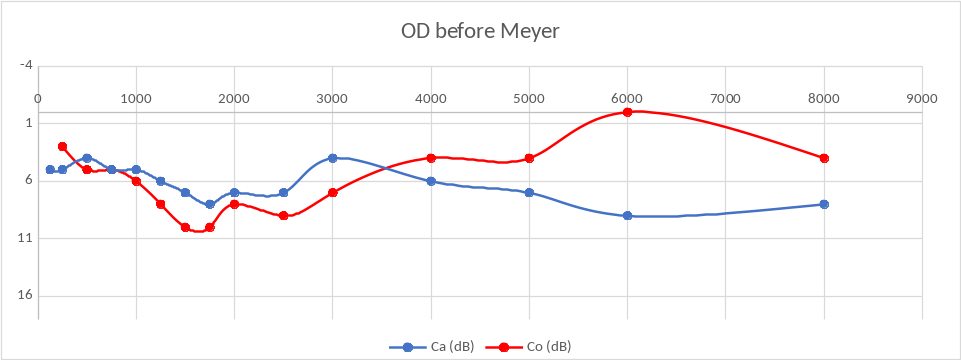
\includegraphics[width=0.7\linewidth]{images/clinique/od_before_meyer.png}
 		\caption{Test d'écoute avant musicothérapie}
 		\label{fig:odbeforemeyer}
 	\end{figure}
 	
 	\lipsum[1]
 	
 	
 	
 	
 	\begin{figure}
 		\centering
 		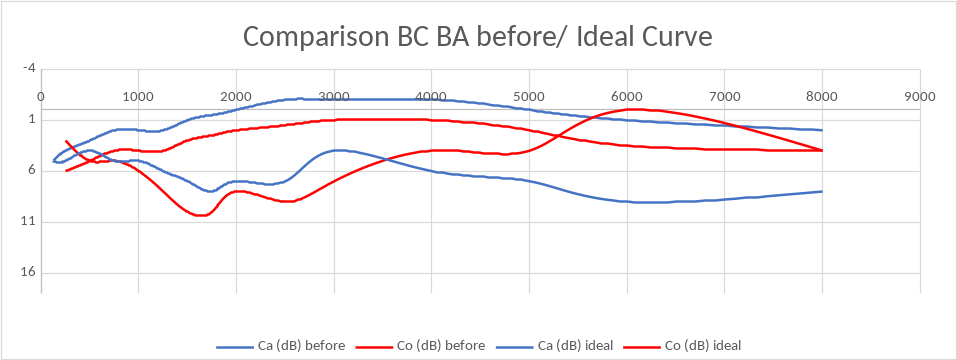
\includegraphics[width=0.7\linewidth]{images/clinique/comparison_bc_ba_before_vs_ideal_curve_meyer.png}
 		\caption[Comparaison avec la courbe idéale]{Comparaison avant
                  musicothérapie des
                  courbes  avec la courbe idéale}
 		\label{fig:comparisonbcbabeforevsidealcurvemeyer}
 	\end{figure}
 	
 	
 	\subsection{Le patient M après la musicoth.}
 	\lipsum[1]
 	\begin{figure}[h]
 		\centering

 		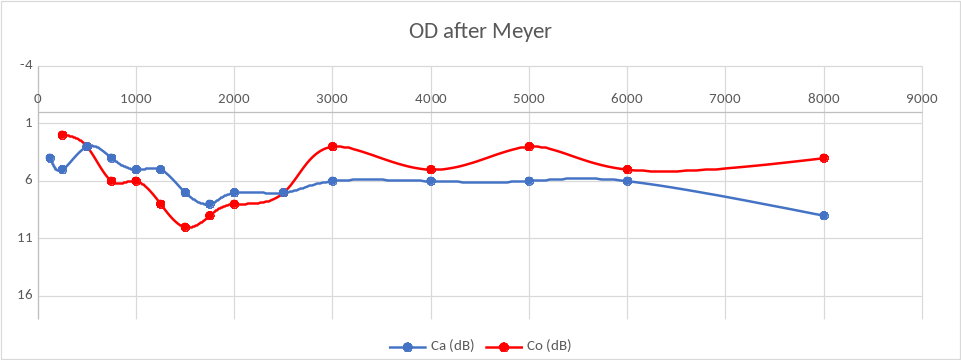
\includegraphics[width=0.7\linewidth]{images/clinique/od_after_meyer.png}
 		\caption{Test d'écoute après la musicothérapie}
 		\label{fig:odaftermeyer}
 	\end{figure}
 
 \lipsum[1]
 
 \begin{figure}[bh]
 	\centering
 	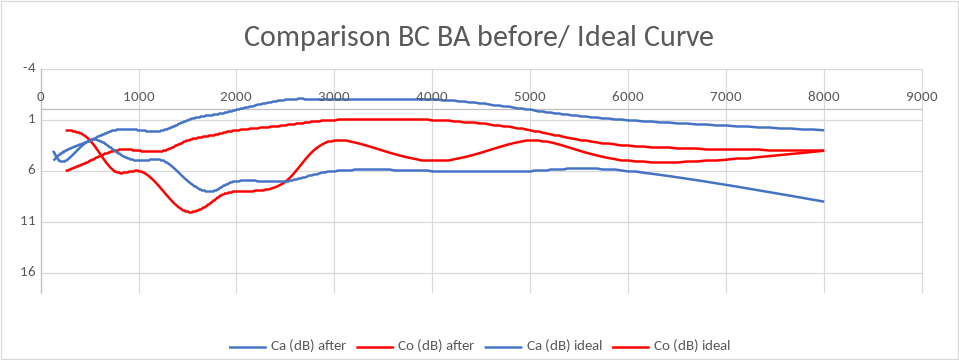
\includegraphics[width=0.7\linewidth]{images/clinique/comparison_bc_ba_after_vs_ideal_curve_meyer.png}
 	\caption{Comparaison avec courbe idéale, après}
 	\label{fig:comparisonbcbaaftervsidealcurvemeyer}
 \end{figure}
 
 





      



 


\section{Graphique:  WHOQO-Bref et Test d'écoute}

Le patient 


\section{Résultats}










   
 

  

  
  


   
   
   
   







\paragraph{Hypothèse}



\paragraph{Y-a-t-il une modification de l'écoute du patient après une prise
en charge en musicothérapie ?}
Est-ce que le processus d'écoute en musicothérapie améliore la capacité
d'écoute ? Devient-elle différente après une musicothérapie?

Est-ce que les test auditifs avant et après la musicothérapie permettent
de visualiser l'action de la musicothérapie?


\paragraph{Est-ce que les résultats ($=$ un changement dans l'écoute) d'une prise
en charge musicothérapeutique peuvent être lisibles et visibles dans
un test d'écoute?}
Est-ce possible d'évaluer un travail musicothérapeutique au moyen
d'un test d'écoute?
Est-ce que ces résultats sont significatifs? 

\paragraph{Est-ce que l'écoute du patient s'est modifié ? si on a pu observer
une modification, dans quel sens va -t-elle ?}

Le contexte: 
est-ce que le contexte est suffisant pour
ressortir des résultats ?





